\documentclass{mcmthesis}
  \makeatletter
  \newcommand{\rmnum}[1]{\romannumeral #1}
  \newcommand{\Rmnum}[1]{\expandafter\@slowromancap\romannumeral #1@}
  \makeatother

\mcmsetup{CTeX = false,   % 使用 CTeX 套装时,设置为 true
        tcn = 91397, problem = C,
        sheet = true, titleinsheet = true, keywordsinsheet = true,
        titlepage = false, abstract = true}
\usepackage{palatino}
\usepackage{lipsum}
\usepackage{cite}
\usepackage{amsmath}  
\usepackage{amssymb}
\usepackage{url}
\usepackage{subfigure}
\usepackage{indentfirst} 
\usepackage{float}

\setlength{\parindent}{1.5em}
\title{}
\begin{document}
\begin{abstract}
abstract
\begin{keywords}
keyword1; keyword2
\end{keywords}
\end{abstract}
\maketitle


\tableofcontents
% \thispagestyle{}% 当前页不显示页码'
\pagestyle{fancy} 
\rhead{\small\sffamily  \rmnum{\thepage}}
\newpage
\pagestyle{fancy}
\rhead{\small\sffamily Page \thepage\ of \pageref{LastPage}}
\setcounter{page}{1}

\section{Introduction}
\subsection{Statement of the problem}
Energy production and energy consumption, which can be regarded as an important economic index, not only reflect the industrial development of a country but also relate to the lifehood of a country. But on the other hand, with the continuous advancement and deepening of the industrialization of human civilization, the consumption of non-renewable energy sources such as coal, petroleum is also accelerating. Hence, the development of cleaner renewable energy is particularly important. After all, if humans depend too much on non-renewable energy sources, the day when fossil fuels are depleted is also a day for humankind to return to agrarian society.

As the world's superpower, many of America's energy policy decentralizes to the state level. to ensure cooperative action between the states\cite{州际契约}, many compacts are formed between states. In this context, along the border with Mexico four states, California, Arizona, new Mexico, Texas hope to form a new energy compact focused on more and more widely used, cleaner renewable energy sources.
\begin{itemize}
  \item Create an energy profile for each of the four states.
  \item Make governors easier to understand the four states’ usage of cleaner, renewable energy sources  and the similarities and difference between the four states.
  \item Determine a state that is appeared to have the ``best" profile for use of cleaner, renewable energy in 2009.
  \item Predict the energy profile of each state in 2025 and 2050.
  \item Determine renewable energy usage targets for 2025 and 2050 which are also for the new four-state energy compact.
  \item Provide at least three suggestions about how to meet the energy compact goals.
\end{itemize}

\subsection{Overview of Our Work}
\begin{itemize}
  \item 
\end{itemize}

\section{Notations and Assumptions}
\subsection{Notations}

\subsection{Assumptions}

\section{Data Processing}

\section{Energy Profile}
\subsection{Overview}

\cite{pr_guide}
\subsection{title}

\subsubsection{Arizona}
\begin{figure}[H]
\begin{minipage}[htb]{0.5\textwidth}
\centering
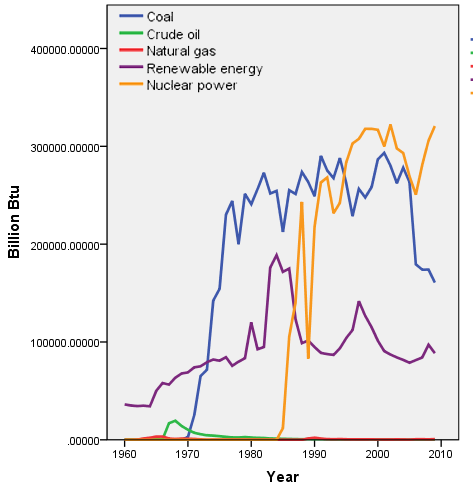
\includegraphics[width=3in]{AZPRB.png}
\caption{AZPRB} \label{fig:AZPRB}
\end{minipage}
\begin{minipage}[htb]{0.5\textwidth}
\centering
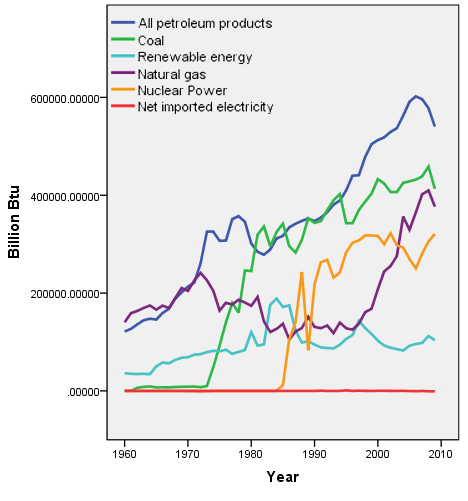
\includegraphics[width=3in]{AZTCB.png}
\caption{AZTCB} \label{fig:AZTCB}
\end{minipage}
\end{figure}

\begin{figure}[H]
\begin{minipage}[htb]{0.5\textwidth}
\centering
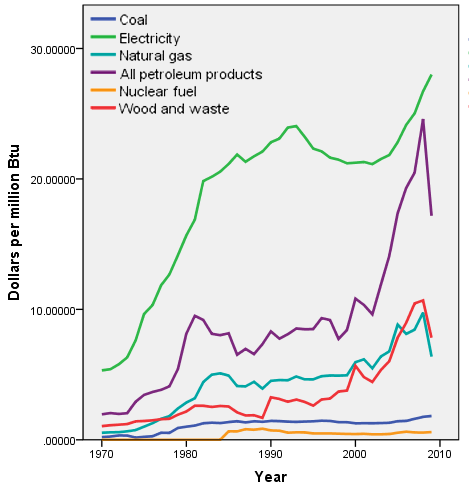
\includegraphics[width=3in]{AZTCD.png}
\caption{AZTCD} \label{fig:AZTCD}
\end{minipage}
\begin{minipage}[htb]{0.5\textwidth}
\centering
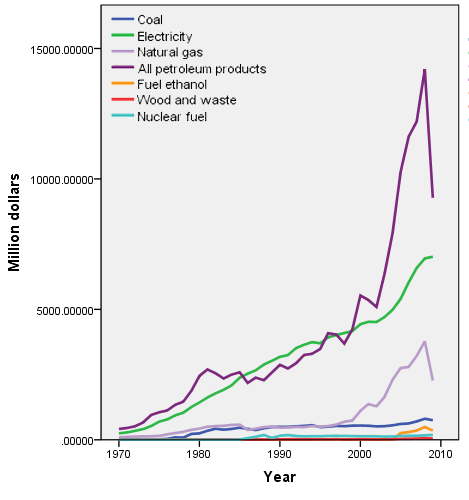
\includegraphics[width=3in]{AZTCV.png}
\caption{AZTCV} \label{fig:AZTCV}
\end{minipage}
\end{figure}

\subsubsection{California}
\begin{figure}[H]
\begin{minipage}[htb]{0.5\textwidth}
\centering
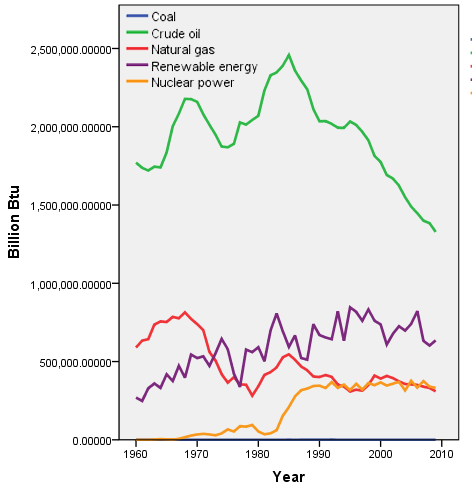
\includegraphics[width=3in]{CAPRB.png}
\caption{CAPRB} \label{fig:CAPRB}
\end{minipage}
\begin{minipage}[htb]{0.5\textwidth}
\centering
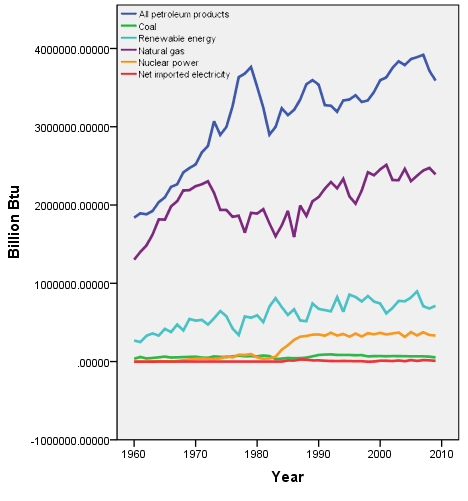
\includegraphics[width=3in]{CATCB.png}
\caption{CATCB} \label{fig:CATCB}
\end{minipage}
\end{figure}

\begin{figure}[H]
\begin{minipage}[htb]{0.5\textwidth}
\centering
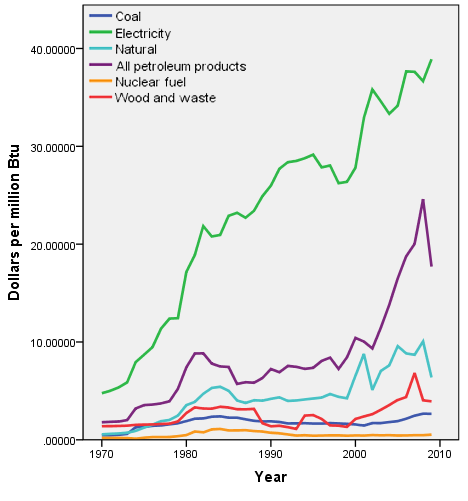
\includegraphics[width=3in]{CATCD.png}
\caption{CATCD} \label{fig:CATCD}
\end{minipage}
\begin{minipage}[htb]{0.5\textwidth}
\centering
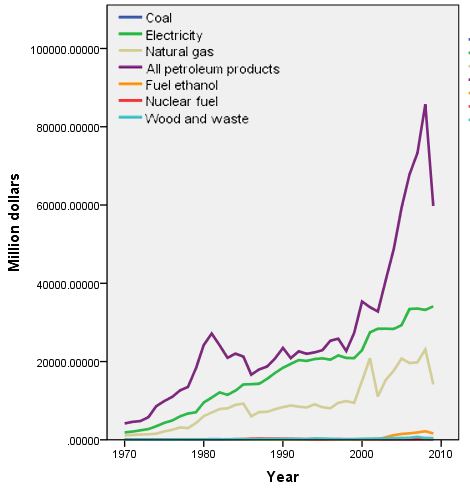
\includegraphics[width=3in]{CATCV.png}
\caption{CATCV} \label{fig:CATCV}
\end{minipage}
\end{figure}

\subsubsection{New Mexico}
\begin{figure}[H]
\begin{minipage}[htb]{0.5\textwidth}
\centering
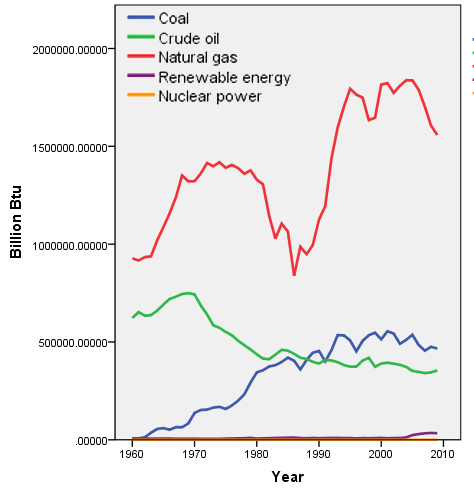
\includegraphics[width=3in]{NMPRB.png}
\caption{NMPRB} \label{fig:NMPRB}
\end{minipage}
\begin{minipage}[htb]{0.5\textwidth}
\centering
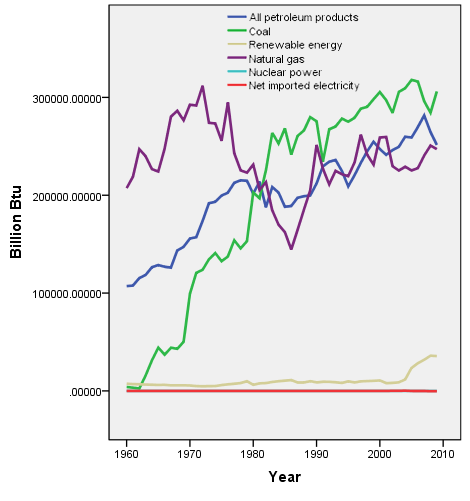
\includegraphics[width=3in]{NMTCB.png}
\caption{NMTCB} \label{fig:NMTCB}
\end{minipage}
\end{figure}

\begin{figure}[H]
\begin{minipage}[htb]{0.5\textwidth}
\centering
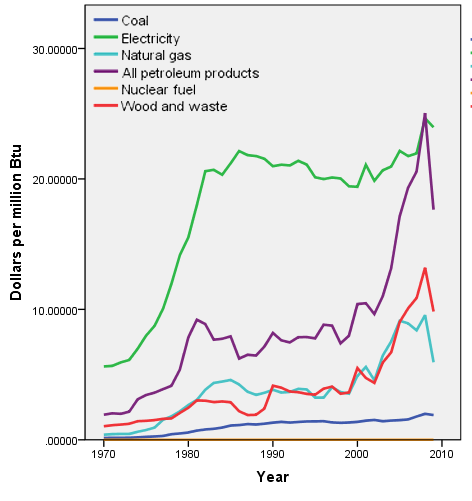
\includegraphics[width=3.in]{NMTCD.png}
\caption{NMTCD} \label{fig:NMTCD}
\end{minipage}
\begin{minipage}[htb]{0.5\textwidth}
\centering
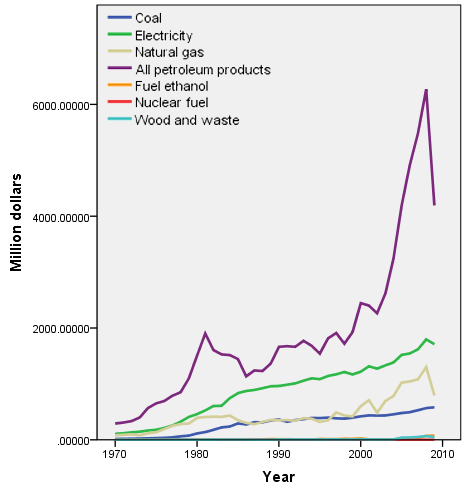
\includegraphics[width=3in]{NMTCV.png}
\caption{NMTCV} \label{fig:NMTCV}
\end{minipage}
\end{figure}

\subsubsection{Texas}
\begin{figure}[H]
\begin{minipage}[htb]{0.5\textwidth}
\centering
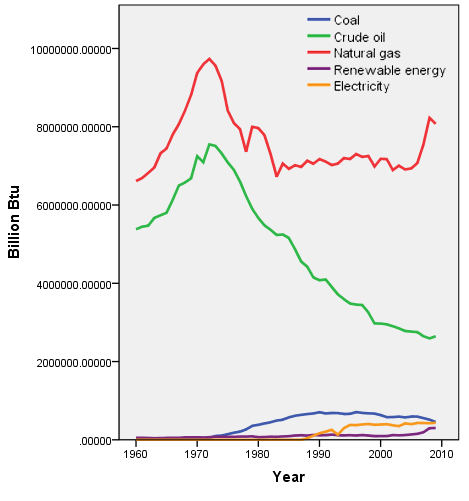
\includegraphics[width=3in]{TXPRB.png}
\caption{TXPRB} \label{fig:TXPRB}
\end{minipage}
\begin{minipage}[htb]{0.5\textwidth}
\centering
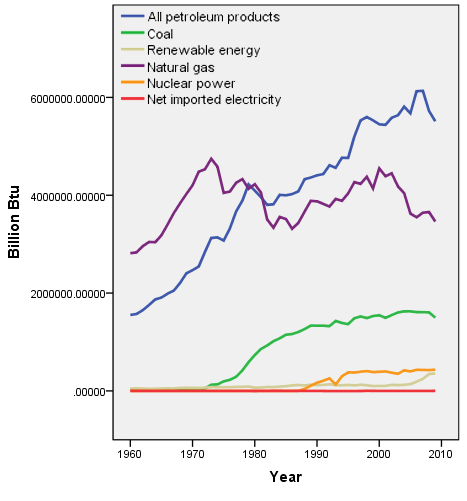
\includegraphics[width=3in]{TXTCB.png}
\caption{TXTCB} \label{fig:TXTCB}
\end{minipage}
\end{figure}

\begin{figure}[H]
\begin{minipage}[htb]{0.5\textwidth}
\centering
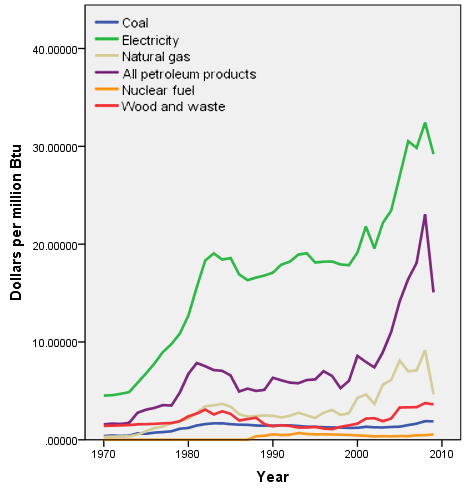
\includegraphics[width=3in]{TXTCD.png}
\caption{TXTCD} \label{fig:TXTCD}
\end{minipage}
\begin{minipage}[htb]{0.5\textwidth}
\centering
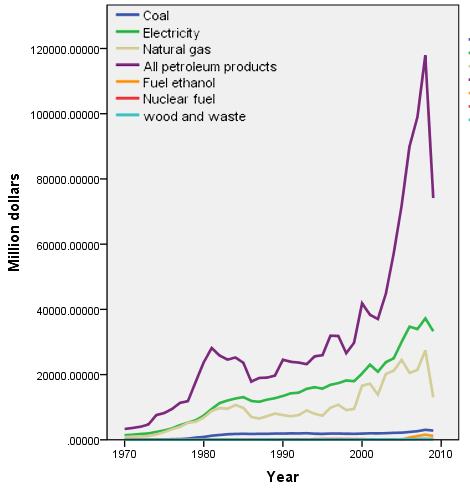
\includegraphics[width=3in]{TXTCV.png}
\caption{TXTCV} \label{fig:TXTCV}
\end{minipage}
\end{figure}






\newpage
\setcounter{page}{2}
\pagestyle{fancy} 
\rhead{\small\sffamily  \rmnum{\thepage}}

\bibliographystyle{siam}
\bibliography{ref}



\begin{appendices}


\begin{minipage}{\textwidth}
  \begin{minipage}[t]{0.45\textwidth}
    \centering
      \makeatletter\def\@captype{table}\makeatother\caption{txCO2}
      \begin{tabular}{|l|c|}
        \hline
        date & million metric tons of CO2 \\ \hline
        1980 & 496.5                      \\ \hline
        1981 & 483.4                      \\ \hline
        1982 & 461.1                      \\ \hline
        1983 & 467.1                      \\ \hline
        1984 & 492.7                      \\ \hline
        1985 & 498.7                      \\ \hline
        1986 & 496.2                      \\ \hline
        1987 & 502.1                      \\ \hline
        1988 & 534.9                      \\ \hline
        1989 & 554.9                      \\ \hline
        1990 & 565.1                      \\ \hline
        1991 & 560.2                      \\ \hline
        1992 & 559.9                      \\ \hline
        1993 & 577.8                      \\ \hline
        1994 & 576.9                      \\ \hline
        1995 & 581.5                      \\ \hline
        1996 & 624.9                      \\ \hline
        1997 & 651.4                      \\ \hline
        1998 & 656.6                      \\ \hline
        1999 & 633.3                      \\ \hline
        2000 & 657.6                      \\ \hline
        2001 & 651.5                      \\ \hline
        2002 & 661.6                      \\ \hline
        2003 & 655.5                      \\ \hline
        2004 & 649.6                      \\ \hline
        2005 & 612.2                      \\ \hline
        2006 & 623.4                      \\ \hline
        2007 & 620                        \\ \hline
        2008 & 585                        \\ \hline
        2009 & 550.1                      \\ \hline
        2010 & 582.5                      \\ \hline
        2011 & 601.5                      \\ \hline
        2012 & 596.3                      \\ \hline
        2013 & 623                        \\ \hline
        2014 & 625.3                      \\ \hline
        2015 & 625.8                      \\ \hline
        \end{tabular}
    \end{minipage}
    \begin{minipage}[t]{0.45\textwidth}
    \centering
          \makeatletter\def\@captype{table}\makeatother\caption{nmCO2}
          \begin{tabular}{|l|c|}
            \hline
            date & million metric tons of CO2 \\ \hline
            1980 & 44.9                       \\ \hline
            1981 & 44                         \\ \hline
            1982 & 45.1                       \\ \hline
            1983 & 48.6                       \\ \hline
            1984 & 46.2                       \\ \hline
            1985 & 46.5                       \\ \hline
            1986 & 43                         \\ \hline
            1987 & 46.2                       \\ \hline
            1988 & 47.9                       \\ \hline
            1989 & 50.4                       \\ \hline
            1990 & 53.3                       \\ \hline
            1991 & 49.2                       \\ \hline
            1992 & 51.7                       \\ \hline
            1993 & 52.6                       \\ \hline
            1994 & 52.5                       \\ \hline
            1995 & 51.1                       \\ \hline
            1996 & 52.6                       \\ \hline
            1997 & 56                         \\ \hline
            1998 & 55.5                       \\ \hline
            1999 & 56.4                       \\ \hline
            2000 & 58.2                       \\ \hline
            2001 & 58.3                       \\ \hline
            2002 & 55.3                       \\ \hline
            2003 & 57.6                       \\ \hline
            2004 & 58.7                       \\ \hline
            2005 & 59.3                       \\ \hline
            2006 & 59.8                       \\ \hline
            2007 & 59                         \\ \hline
            2008 & 56.4                       \\ \hline
            2009 & 57.3                       \\ \hline
            2010 & 53.3                       \\ \hline
            2011 & 55.7                       \\ \hline
            2012 & 53.6                       \\ \hline
            2013 & 53.2                       \\ \hline
            2014 & 50.1                       \\ \hline
            2015 & 50.2                       \\ \hline
            \end{tabular}
  \end{minipage}
\end{minipage}

\begin{minipage}{\textwidth}
  \begin{minipage}[t]{0.45\textwidth}
   \centering
      \makeatletter\def\@captype{table}\makeatother\caption{caCO2}
      \begin{tabular}{|l|c|}
        \hline
        date & million metric tons of CO2 \\ \hline
        1980 & 348.4                      \\ \hline
        1981 & 337                        \\ \hline
        1982 & 299.9                      \\ \hline
        1983 & 293                        \\ \hline
        1984 & 319.5                      \\ \hline
        1985 & 324.2                      \\ \hline
        1986 & 309.5                      \\ \hline
        1987 & 340.1                      \\ \hline
        1988 & 348.2                      \\ \hline
        1989 & 363.5                      \\ \hline
        1990 & 363.9                      \\ \hline
        1991 & 351.7                      \\ \hline
        1992 & 356.1                      \\ \hline
        1993 & 345.5                      \\ \hline
        1994 & 362.4                      \\ \hline
        1995 & 351.4                      \\ \hline
        1996 & 350.5                      \\ \hline
        1997 & 353                        \\ \hline
        1998 & 363.4                      \\ \hline
        1999 & 367                        \\ \hline
        2000 & 382.4                      \\ \hline
        2001 & 386.9                      \\ \hline
        2002 & 386.1                      \\ \hline
        2003 & 373.8                      \\ \hline
        2004 & 392.3                      \\ \hline
        2005 & 389.3                      \\ \hline
        2006 & 397.5                      \\ \hline
        2007 & 402.5                      \\ \hline
        2008 & 385.7                      \\ \hline
        2009 & 372                        \\ \hline
        2010 & 365.9                      \\ \hline
        2011 & 352.2                      \\ \hline
        2012 & 357.1                      \\ \hline
        2013 & 359.8                      \\ \hline
        2014 & 356.7                      \\ \hline
        2015 & 363.5                      \\ \hline
        \end{tabular}
   \end{minipage}
   \begin{minipage}[t]{0.45\textwidth}
    \centering
         \makeatletter\def\@captype{table}\makeatother\caption{azCO2}
         \begin{tabular}{|l|c|}
          \hline
          date & million metric tons of CO2 \\ \hline
          1980 & 52.7                       \\ \hline
          1981 & 59.6                       \\ \hline
          1982 & 58.2                       \\ \hline
          1983 & 53.9                       \\ \hline
          1984 & 58.2                       \\ \hline
          1985 & 60.7                       \\ \hline
          1986 & 55.9                       \\ \hline
          1987 & 56.1                       \\ \hline
          1988 & 59.3                       \\ \hline
          1989 & 65.2                       \\ \hline
          1990 & 62.8                       \\ \hline
          1991 & 63.7                       \\ \hline
          1992 & 66.5                       \\ \hline
          1993 & 69                         \\ \hline
          1994 & 71.7                       \\ \hline
          1995 & 66.7                       \\ \hline
          1996 & 68.4                       \\ \hline
          1997 & 71.6                       \\ \hline
          1998 & 76.5                       \\ \hline
          1999 & 80.4                       \\ \hline
          2000 & 86.1                       \\ \hline
          2001 & 88.4                       \\ \hline
          2002 & 87.8                       \\ \hline
          2003 & 89.6                       \\ \hline
          2004 & 96.6                       \\ \hline
          2005 & 96.7                       \\ \hline
          2006 & 99.9                       \\ \hline
          2007 & 101.9                      \\ \hline
          2008 & 102.3                      \\ \hline
          2009 & 93.4                       \\ \hline
          2010 & 95.2                       \\ \hline
          2011 & 93.3                       \\ \hline
          2012 & 91.3                       \\ \hline
          2013 & 95.1                       \\ \hline
          2014 & 93.1                       \\ \hline
          2015 & 90.9                       \\ \hline
          \end{tabular}
    \end{minipage}
 \end{minipage}




\begin{proof}   %插入证明
  x
\end{proof}

\newtheorem{lemma}{Lemma}%只需在第一个引理开始之前出现一次  
\begin{lemma}  
If $f\in C_{L}^{1,1}(\mathbb{R}^{n})$, then $\forall \textbf{x},\textbf{y}\in\mathbb{R}^{n}$ we have  
\begin{equation}  
\left|{f(\textbf{y})-f(\textbf{x})-\nabla f(\textbf{x})^{T}(\textbf{y}-\textbf{x})}\right|\le\frac{L}{2}\left\|{\textbf{y}-\textbf{x}}\right\|^{2}.  
%\label{eq:eq5}  
\end{equation}  
%\label{lem:lem1}  
\end{lemma} 
\section{First appendix}

\lipsum[13]

% 代码插入
Here are simulation programmes we used in our model as follow.\\

\textbf{\textcolor[rgb]{0.98,0.00,0.00}{Input matlab source:}}
\lstinputlisting[language=Matlab]{./code/mcmthesis-matlab1.m}

\section{Second appendix}

some more text \textcolor[rgb]{0.98,0.00,0.00}{\textbf{Input C++ source:}}
\lstinputlisting[language=C++]{./code/mcmthesis-sudoku.cpp}

\end{appendices}
\end{document}

